\documentclass[12pt]{article}

\input preamble

\title{Principles of Parallel Architecture\\
Homework 1: Parallel Benchmarks}
\author{Xitong Liu \\
xliu@ece.udel.edu}

\begin{document}

\maketitle

\section{Question 1}
[35\%] The TOP 500 is a widely recognized organization that lists the 500 
supercomputers with the most performance in terms of absolute computational 
rate and computational efficiency. Please visit the TOP 500 website: 
\texttt{http://www.top500.org/} and navigate through the site to learn about 
TOP 500.

\begin{enumerate}

\item
\begin{description}
\item[Q: ]According to what the performance is measured? How often the 
rank is updated?
\item[A:]The performance is measured by their performance on the LINPACK 
Benchmark. The rank is updated twice a year.
\end{description}

\item
\begin{description}
\item[Q: ]Plot the performance of the fastest supercomputer vs time since 
1993. What can you comment on this plot?
\item[A: ]According to Fig.\ref{fig:fatest}, 
\begin{figure}[h!]
	\begin{center}
		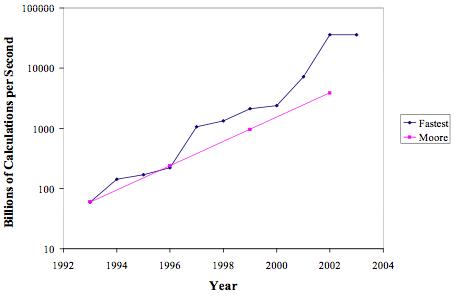
\includegraphics[width=0.7\textwidth, angle=0]{fatest.png}
		\caption{\label{fig:fatest}Fatest SuperComputer in the world}
	\end{center}
\end{figure}
the computing speed doubled roughly every 18 months, following 
the \textbf{Moore's Law}.
\end{description}

\item
\begin{description}
\item[Q: ]Using the statistics tool, generate plots for Architecture, 
Processor Architecture, Processor Family and Number of Processors over 
time. Make conclusions about the progress in these characteristics. 
Where are going the supercomputers according to these characteristics? 
Explain briefly.
\item[A: ]Plots listed as below:
\begin{figure}[h!]
	\begin{center}
		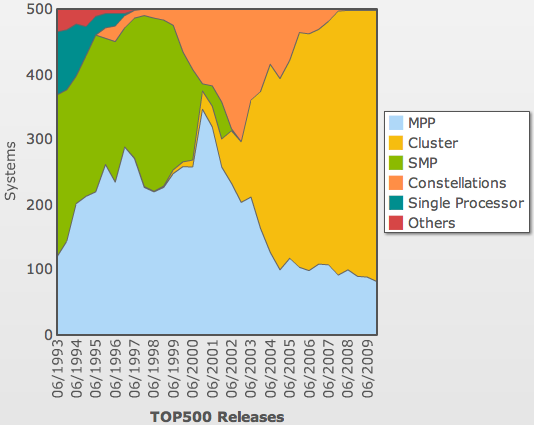
\includegraphics[width=0.7\textwidth, angle=0]{arch-share.png}
		\caption{\label{fig:arch-share}Architecture Share Over Time 1993-2009}
	\end{center}
\end{figure}
\begin{figure}[h!]
	\begin{center}
		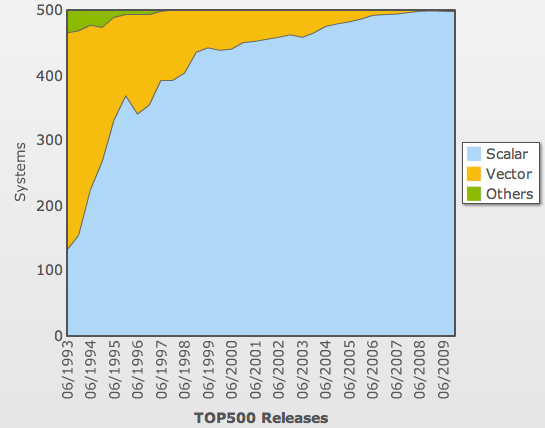
\includegraphics[width=0.7\textwidth, angle=0]{proc-arch-share.png}
		\caption{\label{fig:proc-arch-share}Processor Architecture Share Over Time 1993-2009}
	\end{center}
\end{figure}
\begin{figure}[h!]
	\begin{center}
		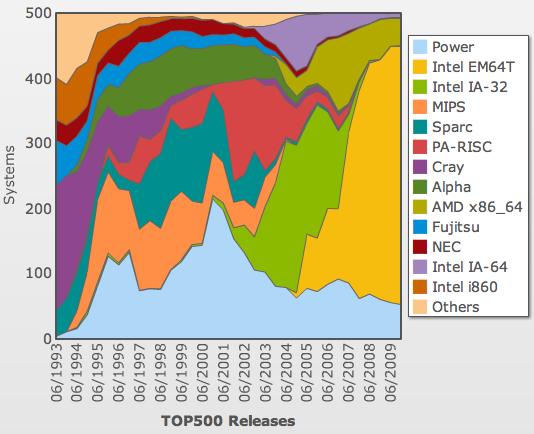
\includegraphics[width=0.7\textwidth, angle=0]{proc-family-share.png}
		\caption{\label{fig:proc-arch-share}Processor Family Share Over Time 1993-2009}
	\end{center}
\end{figure}
\begin{figure}[h!]
	\begin{center}
		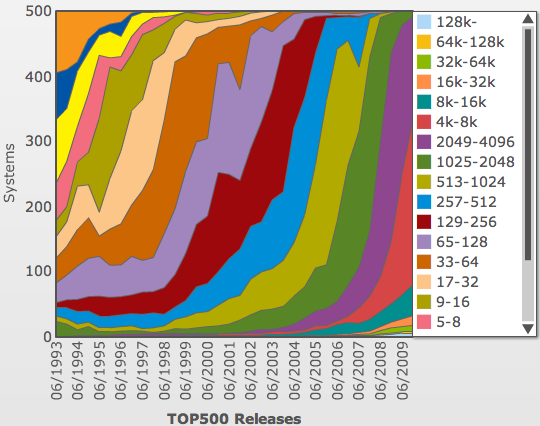
\includegraphics[width=0.7\textwidth, angle=0]{proc-num-share.png}
		\caption{\label{fig:proc-num-share}Number of Processors Share Over Time 1993-2009}
	\end{center}
\end{figure}
As the development of Super Computers, Cluster began to dominate the architecture, 
and most of the processors were scaler based. What's more, Intel EM64T began to 
dominate the processor market in the recent years. The number of processors of one 
super computer bumped dramatically 
in the recent years.
\end{description}

The Green500 provides rankings of the most energy-efficient supercomputers in the 
world. They raise awareness about power consumption, promote alternative total 
cost of ownership performance metrics, and ensure that supercomputers only simulate 
climate change and not create it. Please visit the green 500 website: 
\texttt{http://www.green500.org/}

\item
\begin{description}
\item[Q: ]Plot the computational rate per watt vs time for the top 5 supercomputer 
according to the MFLOPS/W since November 2007. Are they in the top 5 according 
performance? Comment on the evolution of power efficiency of supercomputers.
\item[A: ] See plot
\begin{figure}[h!]
	\begin{center}
		\includegraphics[width=\textwidth, angle=0]{green-top5.pdf}
		\caption{\label{fig:green-top5}Computational Rate Per Watt Over Time 2007-2009}
	\end{center}
\end{figure}
They are not the top5 according to performance. As the development of super computer,
it's more and more energy efficient.

\end{description}

\end{enumerate}

\section{Question 2}
[15\%] Learn how to write a makefile: Write a makefile for the file hello.c that is 
attached. The makefile should have the following rules:

\begin{enumerate}
\item An �all� rule that compiles the program using gcc and generates an executable 
named �hello�
\item A �run� rule that runs the program and redirects its output to the file �out.txt�
\item A �clean� rule that deletes the executable and the output file created by the 
previous rules.
\item Attach the makefile to your homework
\end{enumerate}
Makefile:
\begin{verbatim}
OBJS = hello.o
CC = cc
CFLAGS = -c -g
PROJECT = hello
OUTPUT = out.txt

$(PROJECT) : $(OBJS)
  $(CC) $(OBJS) -o $(PROJECT)

hello.o : hello.c
  $(CC) $(CFLAGS) hello.c

all : $(PROJECT)

run : all
  ./$(PROJECT) > $(OUTPUT)

clean :
  rm -f *.o
  rm -f $(PROJECT)
  rm -f $(OUTPUT)
\end{verbatim}

\section{Question 3}
[50\%] Download the latest version of the Linpack benchmark from\\
\texttt{http://www.netlib.org/benchmark/hpl/}. Compile it:

\begin{enumerate}
\item The tool ``\texttt{find}'', combined with ``\texttt{grep}'' is a good way 
to look for files on directories under Linux. In general, ``\texttt{find | grep xxx}'' 
finds a file that contains \texttt{xxx} in the subdirectories below the current 
directory. Learn how to use ``\texttt{find}'' and ``\texttt{grep}''.
\item Use your knowledge of ``\texttt{find}'' and ``\texttt{grep}'' to find a file 
named ``\texttt{make\_generic}''. Change the permissions of \texttt{make\_generic} so 
that it can be executed.
\item Execute \texttt{make\_generic}. It should create a \texttt{Make.UNKNOWN}
\item In \texttt{Make.UNKNOWN}, set the \texttt{TOPdir} variable to the directory 
where Linpack is.
\item Move \texttt{Make.UNKNOWN} to the Linpack top directory.
\item Make the benchmark using �make�. For this, you will need the MPI runtime and blas 
libraries, if you are working on your machine, you will have to install them, or if you 
are working on a machine that belongs to UDel, please verify that they are available or 
notify the instructor if they are not available so that a solution can be found.
\item Run the tests as specified on the file INSTALL located in the top directory of 
Linpack

Run Linpack. 

The file \texttt{TUNING} has information on how to modify the parameters of the benchmark.

\item Modify the input parameters of the benchmark to get as much performance (GFLOPS) 
as you can. With your report, provide a copy of the parameters you used and the results.
\item Find a range of problem sizes that will be meaningful to analyze the performance 
of a system as a function of problem size.
\item Get a plot of performance as a function of problem size for the parameters 
previously found, for the following systems:
	\begin{enumerate}
		\item \texttt{pacific.capsl.udel.edu}
		\item \texttt{cluster.capsl.udel.edu}
		\item Another computer
	\end{enumerate}
\end{enumerate}
\end{document}